\documentclass[twocolumn]{aastex631}
\usepackage{graphicx}
\usepackage{float}

\begin{document}

\title{Angular Momentum Alignment Between Stellar Remnants and Dark Matter Halos in Galaxy Mergers}
\author{Ben A Phan}
\date{April 11, 2025}

\begin{abstract}
    This project investigates the angular momentum alignment between stellar remnants and their dark matter halos during a major merger, focusing on the MW-M31 interaction. In particular, this work uses low resolution simulation of the MW-M31 system to track the angular momentum vectors of the stellar and halo components of both galaxies, evaluate how their directions evolve relative to their initial orientations, and one another. This will allow us to estimate how a major merger would distort the angular momentum alignment between galaxies' components and whether or not such alignment is re-established in the post-merger structure. The simulation data reveal that\footnote{Data summary of result goes here.} the stellar and halo components begin moderately aligned, become significantly misaligned during the merger, and partially realign post-merger. This analysis provides insight into the dynamics of dark matter about stellar structure in galaxy evolution and whether their angular momentum alignment persists after major merger (violent dynamic interaction?).
\end{abstract}


\keywords{Galaxy --- Galaxy Evolution --- Stellar Disk --- Dark Matter Halo --- Major Merger --- Angular Momentum --- Hernquist Profile --- Dynamical Friction --- Tidal stripping/sharing --- N-body Simulation}

\section{Introduction}


\subsection{Angular Momentum Alignment in Galaxy Merger}
The angular momentum alignment between stellar structures and their surrounding dark matter halos significantly impacts galaxies' formation, structure, and dynamics. According to previous studies (e.g. \cite{Somerville2008, Chua2019, Baptista2023}), galaxy evolution involves complex interactions between baryonic matter and dark matter halos, especially during galaxy mergers when angular momentum is rearranged and realigned. In particular, during this event, angular momentum is redistributed through \textbf{tidal stripping/sharing}—the removal or exchange of weak gravitationally bounded material between interacting galaxies—and \textbf{dynamical friction}, a process where a massive object loses momentum through gravitational interactions with surrounding matter, generating ``friction" or a drag force. These effects often lead to misalignment between the baryonic and dark matter components. 

This study focuses on the Milky Way–Andromeda (MW–M31) system and investigates how the angular momentum vectors of their dark matter halos and stellar disks evolve before, during, and after their \textbf{major merger}, defined as the interaction between two galaxies of comparable mass (typically within a 3:1 mass ratio; \citealt{Lotz2011}). The goal is to determine whether these components realign after coalescence or retain signs of the misalignment due to the dynamical disturbance from the merging event.


\subsection{Significance to Galaxy Evolution}

Understanding the alignment between the \textbf{stellar disk} and \textbf{dark matter halo} angular momentum is essential for interpreting how galaxies form and evolve. A \textbf{galaxy} is a gravitationally bound system of stars whose properties cannot be explained by baryonic matter (i.e., gas, dust, and stars) and Newton's Law of Gravity alone. Instead, it requires the presence of dark matter to match observations \citep{Willman2012}. The \textbf{stellar disk} forms the visible, rotationally supported component of many galaxies, while the \textbf{dark matter halo} is the extended, invisible structure that dominates the total mass and gravitational potential.

\textbf{Galaxy evolution} includes the full range of physical processes—such as mergers, gas accretion, and tidal interactions—that reshape the mass distribution, morphology, and kinematics of a galaxy over cosmic time. These processes not only affect physical properties like stellar mass or gas content, but also play a key role in determining the dynamics between galaxies, such as their angular momentum realignment between components.

A central quantity in this study is the \textbf{angular momentum} vector:
\[
\vec{L} = \sum_i m_i (\vec{r}_i - \vec{r}_{\text{COM}}) \times (\vec{v}_i - \vec{v}_{\text{COM}})
\]
where $m_i$ is the mass of a particle, and $\vec{r}_i$, $\vec{v}_i$ are its position and velocity relative to the component’s center of mass.

Since dark matter cannot be directly observed, to characterize its structure, we apply the \textbf{Hernquist profile}, a radial density model defined as:
\[
\rho(r) = \frac{M}{2\pi} \frac{a}{r(r+a)^3}
\]
where $M$ is the total mass and $a$ is the scale radius. This profile ensures a finite total mass and helps define a stable core for angular momentum measurements \citep{Hernquist1990}.

The alignment between halo and stellar angular momentum affects many observable properties, including galaxy size, morphology, rotation curves, and stellar velocity dispersion. Recent studies, including \citet{Chua2019} and \citet{Baptista2023}, have shown that angular momentum alignment is a valuable tracer of dynamical evolution during and after galaxy mergers.

\subsection{Current Understanding}
Recent studies have significantly improved our understanding on stellar-halo angular momentum alignment. \cite{Somerville2008} demonstrated the importance of realistic dark matter halo models (e.g., NFW profiles and adiabatic contraction) in accurately predicting the weaker observed evolution of galaxies compared to previous prediction model with simpler dark matter profile (see Fig.~\ref{fig:somerville_fig5}). Similarly, \cite{Chua2019} highlighted that stellar and dark matter angular momentum vectors tend to connect more strongly in massive halos at lower redshifts, suggesting this alignment depends on both mass and time. Furthermore, \cite{Baptista2023} showed that evolving stellar-to-halo mass ratios significantly impact the angular momentum distributions, influencing both galaxy formation and evolutionary trajectories.

\begin{figure}[H]
    \centering
    \includegraphics[width=0.45\textwidth]{figure5.png}
    \caption{Evolution of average disk sizes normalized to present-day sizes as a function of redshift, with circles representing more detailed halo profiles. The circles show a more gradual size in evolution, which agrees more with observation. This emphasizes predictions from more realistic dark matter halo models. Adapted from \citet{Somerville2008}.}
    \label{fig:somerville_fig5}
\end{figure}


\subsection{Open Questions}
Despite the significant progress on studying this topic, there are still many unknown questions:
\begin{itemize}
    \item How does angular momentum alignment evolve throughout and after galaxy mergers?
    \item What factors govern the strength and persistence of this alignment throughout galaxy evolution?
    \item How does angular momentum realignment affect the structure and kinematics of stellar remnants post-merger?
\end{itemize}

\section{This Project}

\subsection{Project Overview}

This project investigates the angular momentum alignment between the dark matter halo and stellar disk components of the Milky Way (MW) and Andromeda (M31) galaxies before, during, and after their merger. Using a VLowRes simulation of the Local Group, we track the evolution of angular momentum vectors from $t = 0$ Gyr to approximately $t = 12$ Gyr across 17 time snapshots (spaced at 0.5 Gyr intervals). For each galaxy, we compute the angular momentum of the halo and disk using inner regions—$r < 63$ kpc for the halo, based on the Hernquist scale length, and $r < 15$ kpc for the disk—to minimize biases from fast-moving particles in the loosely-bounded regions. After $t \sim 6.5$ Gyr, when MW and M31 fully coalesce, we calculate the alignment of the merger remnant. This approach allows us to quantitatively assess whether angular momentum realigns post-merger or remains disrupted.

\subsection{Research Question}

This project addresses the open question: \textit{How does angular momentum alignment evolve through a major merger?} Specifically, we examine whether the dark matter halo and stellar disk components of a galaxy maintain, lose, or recover alignment during and after the MW–M31 merger. This question is significant to our understanding of \textbf{galaxy evolution} because the preservation or disruption of angular momentum coherence directly affects disk regrowth, remnant morphology, and kinematic stability. By following the complete timeline of mergers from $t = 0$ to $t \approx 12$ Gyr in the simulation, this study provides a picture of how mergers shape the structure of angular momentum over time. 

\subsection{Method Overview}
This analysis will use the provided MW-M31 simulation data, following these specific methods:

\begin{enumerate}
    \item \textbf{Particle Classification and Mass Distribution} (code used from ReadFile, ParticleProperties, and GalaxyMass functions): Identify halo, disk, and bulge particles for each galaxy, then examine their mass and velocity distributions. This will define the evolving mass distribution and structure throughout the merger.
    
    \item \textbf{Center of Mass Analysis} (code used from CenterOfMass and OrbitCOM functions): Calculate the COM positions and velocities for each galaxy at different simulation snapshots, establishing an accurate frame of reference for angular momentum analysis.

    \item \textbf{Angular Momentum Calculation} (code used from Lab 3): Compute the angular momentum vectors of stellar and dark matter halo particles separately. This calculation will use each galaxy’s COM frame, determined by subtracting the galaxy’s COM position and velocity from particle positions and velocities. The angular momentum vectors' magnitudes and directions will be tracked across simulation snapshots, allowing analysis of alignment evolution throughout the merger process.

    \item \textbf{Galaxy Morphology and Shape Evolution} (code used from Lab 6 and Lab 7): Apply contour plots to quantify changes in halo and stellar morphology, demonstrating the impact of mergers on the shape of the galaxy and its halo.
\end{enumerate}

\section{Methodology}

\subsection{Simulation Overview}

We use the VLowRes Local Group simulation provided by the ASTR400B course\footnote{Citation for the simulation paper will be added here since I don't know what the paper is.}, which models the gravitational evolution of the Milky Way (MW) and Andromeda (M31) galaxies through their eventual merger.


This is an example of an \textbf{N-body simulation} which follows the evolution of a system of collisionless particles under their mutual gravitational forces \citep{Springel2005}. In this case, particles represent dark matter and stellar mass distributions in each galaxy.

Each galaxy is initially modeled as:
\begin{itemize}
    \item Type 1: \textbf{Dark matter halo} particles, following a \textbf{Hernquist profile} \citep{Hernquist1990}, with scale radius $a \approx 63$ kpc. This density profile provides total mass and replicates the inner structure of observed halos by modeling the radial mass distribution in three-dimensional space using spherical coordinates.
.
    \item Type 2: \textbf{Stellar disk} particles, selected within a radial cutoff of $r < 15$ kpc to focus on the rotationally supported baryonic structure. This simulation also includes a similar data set to the dark matter halo particles.
\end{itemize}

The simulation provides outputs at 800 Myr intervals, including particle data snapshots and orbital tracking files. The initial halo masses are $M_{\text{MW}} \sim 10^{12} M_\odot$ and $M_{\text{M31}} \sim 1.6 \times 10^{12} M_\odot$, providing sufficient resolution to track angular momentum evolution throughout the merger.


\subsection{Step-by-Step Procedure}

\begin{enumerate}
    \item \textbf{Read Data}: Load particle positions, velocities, and types for each snapshot using `ReadFile.py`.
    \item \textbf{Identify Components}: Select halo (type 1) and disk (type 2) particles.
    \item \textbf{COM Calculation}: Use `CenterOfMass.py` to compute COM position and velocity for each component.
    \item \textbf{Apply Radial Cutoffs}: Use $r < 63$ kpc for halos and $r < 15$ kpc for disks.
    \item \textbf{Compute Angular Momentum}: Calculate $\vec{L}$ for each component using the COM frame.
    \item \textbf{Track Angular Momentum Evolution}: For each snapshot, calculate the angle between the component's angular momentum vector and its original direction at snapshot 0. This measures how much the halo and disk have reoriented over time.

    \item \textbf{Compare Halo vs. Disk Alignment}: Measure misalignment angle between halo and disk components over time.
    
   \item \textbf{Post-Merger Analysis}: After $t \sim 6$ Gyr, when MW and M31 have merged, combine the halo and disk particles from both galaxies to compute the angular momentum vectors of the merger remnant. This includes calculating a new center of mass for the combined system and tracking the evolution of halo–disk alignment in the post-merger structure.

\end{enumerate}

\subsection{Figures}

\begin{figure}[ht!]
    \centering
    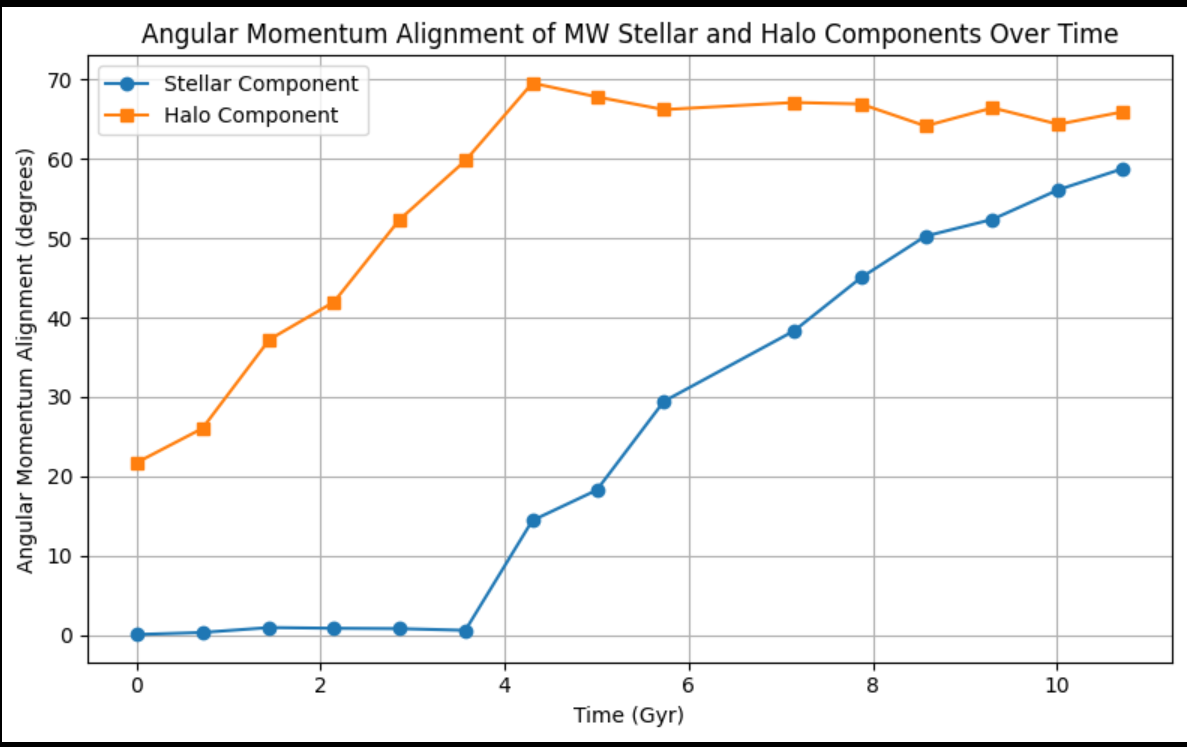
\includegraphics[width=0.45\textwidth]{MW_Angular_Momentum_Alignment_Time.png}
    \caption{MW halo and disk angular momentum vectors tracked over time relative to their directions at snapshot 0.}
    \label{fig:mw_vector_evolution}
\end{figure}

\begin{figure}[ht!]
    \centering
    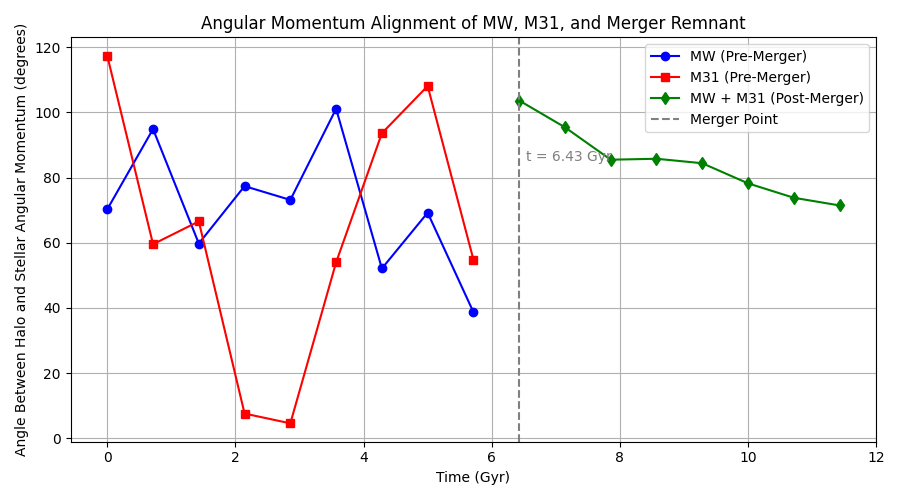
\includegraphics[width=0.45\textwidth]{Angular_Momentum_MW_M31_Merger.png}
    \caption{Angle $\theta$ between halo and stellar angular momentum for MW, M31, and the merger remnant.}
    \label{fig:misalignment_plot}
\end{figure}

\subsection{Calculations and Plot Interpretation}

The main calculation performed in this project is the angular momentum vector of a group of particles (either halo or disk), defined by:
\[
\vec{L} = \sum_i m_i (\vec{r}_i - \vec{r}_{\text{COM}}) \times (\vec{v}_i - \vec{v}_{\text{COM}})
\]
where $m_i$ is the mass of particle $i$, and $\vec{r}_i$ and $\vec{v}_i$ are the position and velocity vectors relative to the system’s center of mass (COM). This equation computes the total angular momentum of each component in a COM frame. COM values are calculated iteratively via the shrinking sphere method.

To measure angular momentum evolution, we compare the current vector $\vec{L}_t$ at each snapshot $t$ to the initial direction $\vec{L}_0$ from snapshot 0 using the dot product property:
\[\theta_t = \cos^{-1}\left( \frac{ \vec{L}_t \cdot \vec{L}_0 }{ |\vec{L}_t||\vec{L}_0| } \right)\]
This angle $\theta_t$ shows how much the vector has rotated over time.

Similarly, to evaluate halo–disk coupling at each snapshot, we compute:
\[\phi_t = \cos^{-1}\left( \frac{ \vec{L}_\text{halo} \cdot \vec{L}_\text{disk} }{ |\vec{L}_\text{halo}||\vec{L}_\text{disk}| } \right)\]
where $\phi_t$ is the misalignment between halo and stellar angular momentum directions. If $\phi_t$ remains low, halo–disk alignment is preserved. Large $\phi_t$ indicates kinematic decoupling during the merger.

The two diagnostic plots generated from these calculations are:
\begin{itemize}
    \item \textbf{Figure 1:} Angular momentum angle $\theta_t$ relative to the initial vector ($\vec{L}_0$) for MW’s halo and stellar disk. This plot reveals how much the orientation of each component changes over time.
    \item \textbf{Figure 2:} Instantaneous halo–disk angle $\phi_t$ for MW, M31, and the post-merger remnant. This allows us to see when halo–disk coupling weakens, and whether it recovers.
\end{itemize}

Together, these (incompleted) calculations and plots quantify the timing and extent of angular momentum misalignment during a major merger, providing direct insight into post-merger dynamics and structure.

\subsection{Hypothesis}

We hypothesize that:
\begin{itemize}
    \item MW and M31 start with moderate halo–disk alignment.
    \item \textbf{Dynamical friction} and tidal interactions during the merger disrupt this alignment.
    \item After coalescence, partial realignment occurs, but full restoration of coherence is unlikely.
\end{itemize}

\bibliography{cite.bib}
\bibliographystyle{aasjournal}

\end{document}